\chapter{Motorselectie}
% Inhoud volgt
Nu gaan we kijken naar hoe we kunnen bepalen welke motor we nodig hebben voor een bepaalde
toepassing.
Dit kan afhangen van applicatie, beschikbare catalogus, standaarden (normen, vind je ook
op kenplaat zoals bvb.
IEC 60034), dimensionering, $\cdots$

\begin{figure}[H]
  \centering
  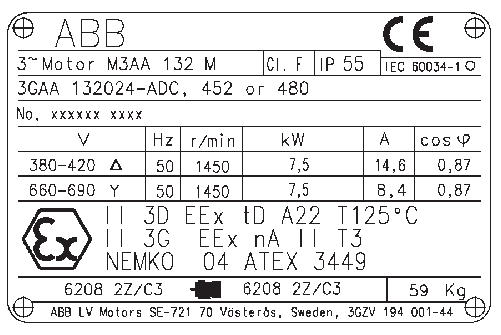
\includegraphics[width=0.6\textwidth]{assets/kenplaatmetnorm.png}
  \caption{Kenplaat met norm IEC 60034}
  \label{fig:kenplaatmetnorm.png}
 \end{figure}

Op deze kenplaat zien we vanalle dingen die we zometeen nog verder zullen bespreken, ik
wil het nu even hebben over die IEC 60034, dit is een norm van de \textbf{Internationale
Elektrotechnische Commitee}, zij hebben normen over zo goed als alles wat elektrisch is
zoals bvb.
energiecurves en efficiëntieklassen.
Er is ook nog een Amerikaanse versie, hier hebben we het al eerder over gehad, namelijk de
\textbf{NEMA}.

\begin{figure}[H]
  \centering
  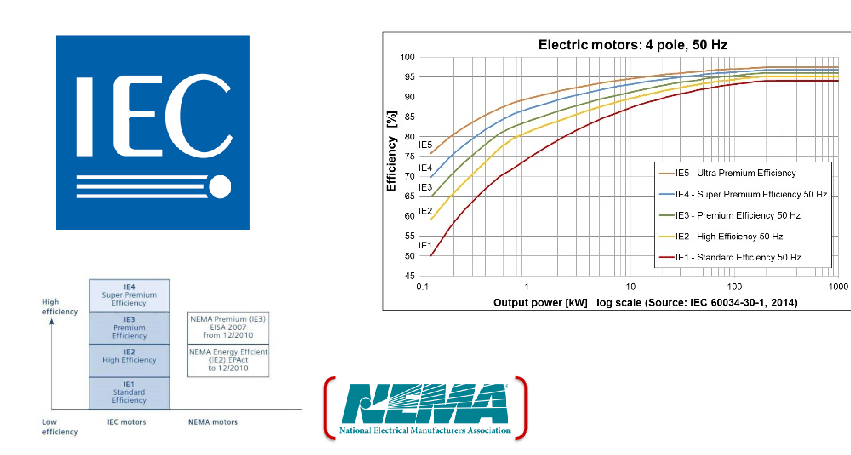
\includegraphics[width=0.6\textwidth]{assets/standaarden.png}
  \caption{IEC en NEMA}
  \label{fig:standaarden.png}
 \end{figure}

\subsection{IP-klasse}
Iets wat we eigelijk al veel hebben gezien maar hier dus ook voorkomt zijn de zogenaamde
IP-klassen, IP staat voor \textit{Index of Protection}.
Een IP-klasse is altijd een nummer met 2 cijfers, het eerste cijfer toont de bescherming
tegen vaste voorwerpen en het tweede cijfer de bescherming tegen vloeistoffen.
Hoe hoger het cijfer hoe beter de bescherming.
Hier is een overzicht van de IP-klassen:

\begin{figure}[H]
  \centering
  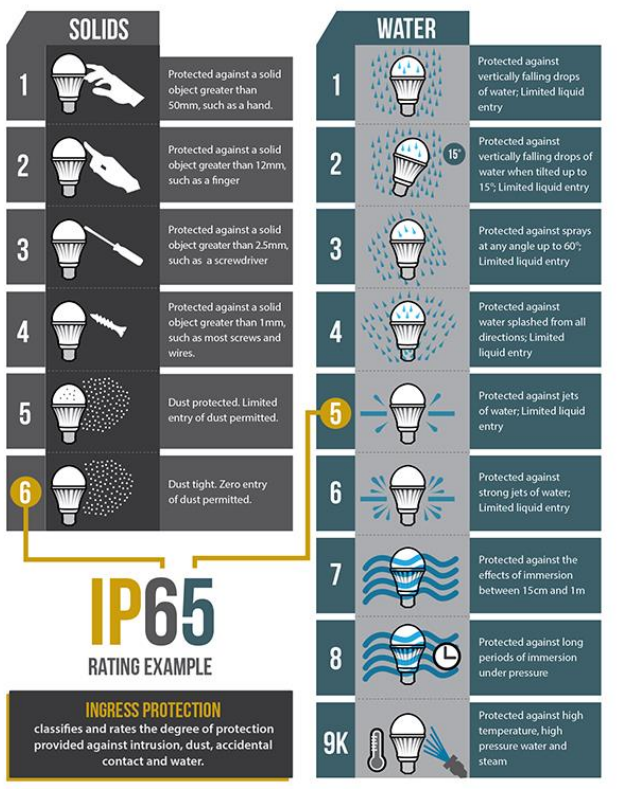
\includegraphics[width=0.4\textwidth]{assets/IPklassennummers.png}
  \caption{IP-klassen}
  \label{fig:IPklassennummers.png}
 \end{figure}

Een IP23 zoals de gele motor is dan dus bescherm tegen iets grotere voorwerpen, dus je
vingers kunnen er niet tussen maar lucht en stof kan dus binnen.
Een IP55 zoals de blauwe motor is juist helemaal dicht en kan tegen waterstralen.

\begin{figure}[H]
  \centering
  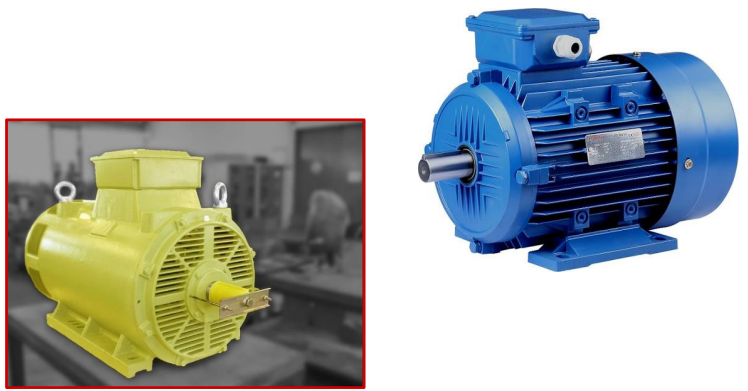
\includegraphics[width=0.5\textwidth]{assets/geleenblauwemotor.png}
  \caption{Gele en blauwe motor met IP23 en IP55}
  \label{fig:geleenblauwemotor.png}
 \end{figure}

\subsection{Isolatieklassen}
Ook hebben we isolatieklassen, deze duiden aan hoe warm de isolatie van de motor mag
worden (op nominale stroom).
Dit is belangrijk om zicht over te hebben want materiaal verouderd bij hogere
temperaturen.
Deze klassen worden opgesteld door te kijken naar welk onderdeel van de machine het eerste
faalt, want brand willen we absoluut vermijden.
De onderstaande grafiek toont de maximale temperaturen (voor op nominale stroom) dat je
machine mag worden bij die bepaalde klasse (A,E,B,F,H) met H de beste dus.

\begin{figure}[H]
  \centering
  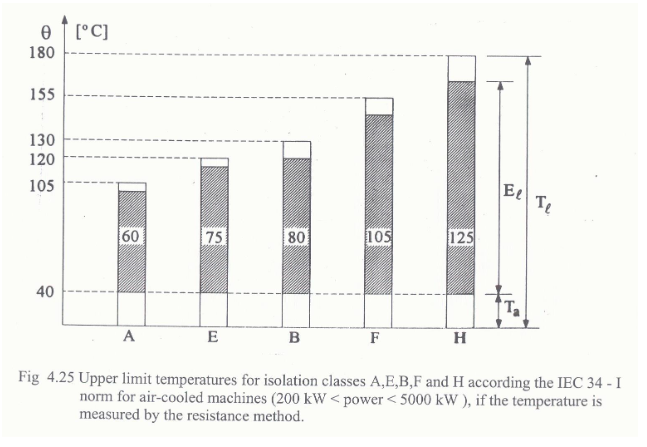
\includegraphics[width=0.6\textwidth]{assets/isolatieklassen.png}
  \caption{Isolatieklassen}
  \label{fig:isolatieklassen.png}
 \end{figure}

\subsection{Nominaal werkingspunt vs. echt werkingspunt}
{\color{red}(Dit stukje is deels door AI geschreven op basis van mijn lesnotities, ik heb
nagekeken en het klopt allemaal en is effectief allemaal aan bod gekomen in de les)}

Voor motorselectie kijk je best niet alleen naar het nominaal werkingspunt op de kenplaat,
want in de praktijk draait de motor vaak op een lagere belasting (echt werkingspunt).
Zowel het rendement als de arbeidsfactor zijn namelijk geen constante kenplaatwaarden,
maar hangen sterk af van de belastingsgraad.
Bij nullast geldt $\eta=P_{mech}/P_{el}\to 0$:
er is geen nuttig mechanisch vermogen ($P_{mech}=0$), maar wel nog steeds verliezen
(ijzer-, wrijvings- en magnetiseerverliezen), dus $P_{el}>0$.
De arbeidsfactor daalt echter veel sterker bij deellast dan het rendement.
Dit komt doordat het reactief vermogen $Q$ (nodig voor de magnetisatie, via $X_m$)
nauwelijks verandert met de belasting, terwijl het actief vermogen $P$ wel sterk daalt.
Aangezien $\cos\varphi=P/S=P/\sqrt{P^2+Q^2}$, zakt $\cos\varphi$ hierdoor snel naarmate de
belasting afneemt (tot ongeveer $0{,}2-0{,}4$ bij nullast).
Dit is dan ook een belangrijke reden om een motor niet te overdimensioneren:
bij een motor die permanent ver onder zijn nominaal vermogen draait, zakt de arbeidsfactor
sterk, wat extra reactief vermogen van het net vraagt zonder bijkomend nuttig vermogen.
Op de volgende grafiek zien we dan hoe het rendement en de arbeidsfactor afnemen naarmate
de motor meer belast wordt, dit is dus uitgezet met een verticale reductiecoëficiënt:

\begin{figure}[H]
  \centering
  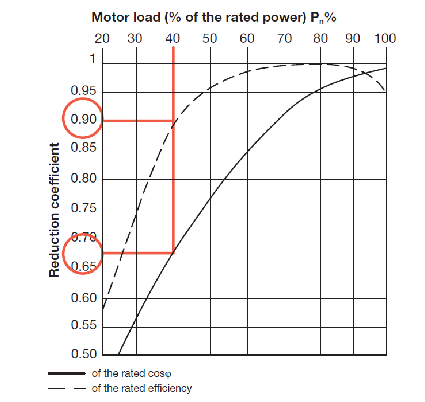
\includegraphics[width=0.4\textwidth]{assets/reductierendementenarbeidsfactor.png}
  \caption{Grafiek reductie van rendement en arbeidsfactor bij deellast}
  \label{fig:reductierendementenarbeidsfactor.png}
 \end{figure}

Het rendement is hier eigelijk uitgedrukt als $\frac{\eta}{\eta_{nom}}$ en de
arbeidsfactor als $\frac{\cos\varphi}{\cos\varphi_{nom}}$.
Wat we dus ook zien is dat het rendement naar 0 gaat bij nullast.
En in het begin de snelheid het hoogste is, het is dus hoger bij deellast dan vollast.

\subsection{Werkingsregimes of Intermiteair gedrag}
Dan kunnen we ook nog classificeren hoe de motor belast kan worden in de tijd, wat bepaalt
hoe de motor moet worden gekoeld of gewoon tot hoelang de motor kan werken.
Classificaties hiervan worden aangeduid met S en dan een getal erachter van S1 tot S8, een
paar voorbeelden zijn in de les gezien en zal ik nu overlopen.

\begin{figure}[H]
  \centering
  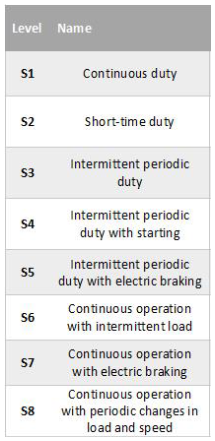
\includegraphics[width=0.25\textwidth]{assets/werkingsregimes.png}
  \caption{Werkingsregimes klassen S1 tot S8}
  \label{fig:werkingsregimes.png}
 \end{figure}

Klasse S1 ziet er als volgt uit:

\begin{figure}[H]
  \centering
  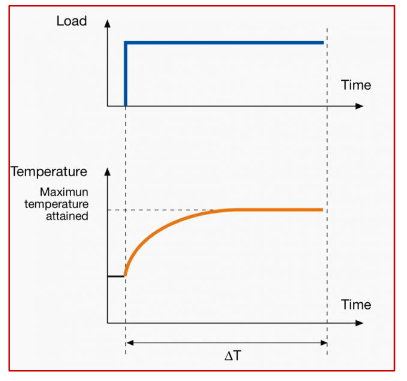
\includegraphics[width=0.35\textwidth]{assets/S1.png}
  \caption{S1 werkingsregime}
  \label{fig:S1.png}
 \end{figure}

Hier zet je de motor aan en laat je hem aan staan op het zelfde vermogen, het duurt even
tot de temperatuur op regimetemperatuur komt maar daarna veranderd die niet, deze klasse
kan dus gewoon constant blijven in de tijd.
In de onderstaande figuur de S3 klasse:

\begin{figure}[H]
  \centering
  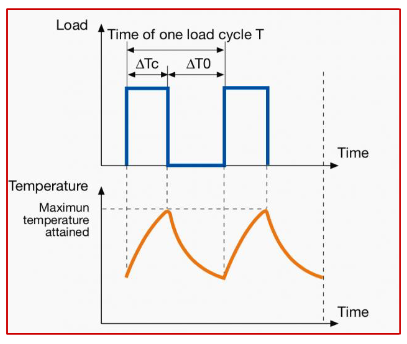
\includegraphics[width=0.35\textwidth]{assets/S3.png}
  \caption{S3 werkingsregime}
  \label{fig:S3.png}
 \end{figure}

Wat we hier dan zien is dat we de motor aanzetten, deze gaat opwarmen tot een bepaalde
temperatuur en dan gaan we hem uitzetten, hij gaat dan afkoelen.
Dit gaan we dan herhalen, dit kan dus een aantal keer na elkaar.
Het is dus een intermitent gedrag (periodisch), het kan niet constant blijven werken.
En de laatste dat is besproken is dan S4:

\begin{figure}[H]
  \centering
  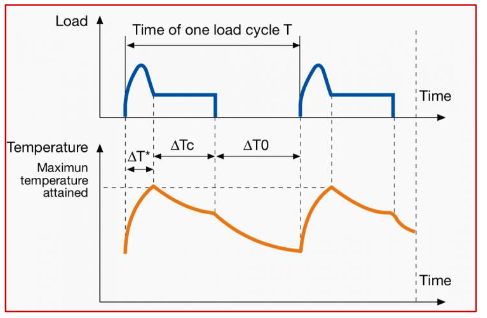
\includegraphics[width=0.4\textwidth]{assets/S4.png}
  \caption{S4 werkingsregime}
  \label{fig:S4.png}
 \end{figure}

Hier was niet echt uitleg over in de les gegeven dus deze ga ik niet in detail verder
bespreken.

\subsection{Explosie veilig materiaal}
Er zijn ook coderingen afhankelijk van je werkingsomgeving, zoals bijvoorbeeld
explosieveilig materiaal.
Dit is belangrijk in de chemische industrie waar er veel gassen en dampen zijn die kunnen
ontbranden.
Hier zijn dan ook speciale motoren voor nodig die dit kunnen weerstaan.
Deze worden aangeduid met een lettercode, deze kan je terugvinden op de kenplaat van de
motor.

\begin{figure}[H]
  \centering
  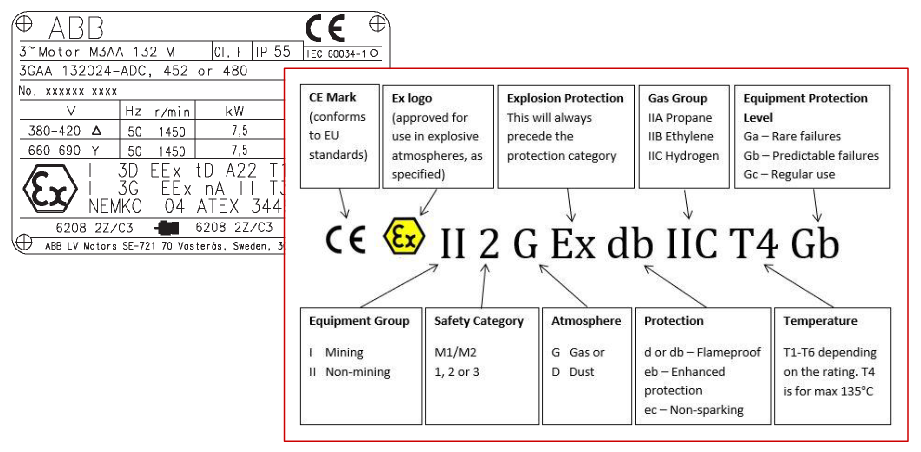
\includegraphics[width=0.6\textwidth]{assets/explosiecodering.png}
  \caption{Explosieveilige codering van motoren}
  \label{fig:explosiecodering.png}
 \end{figure}

\subsection{Bouwvorm}
Bouwvorm is ook iets dat wordt weergegeven op de kenplaat, typisch met een B en dan een
getal voor horizontale assen en een V en een getal voor verticale assen.
Dit is handig want na 15 jaar ofzo kan je dan bvb.
van motor veranderen in je machine en kan je gewoon een motor van een andere type of merk
nemen zolang dat die bouwvorm hetzelfde is, het past dan nog steeds in je machine.

\begin{figure}[H]
  \centering
  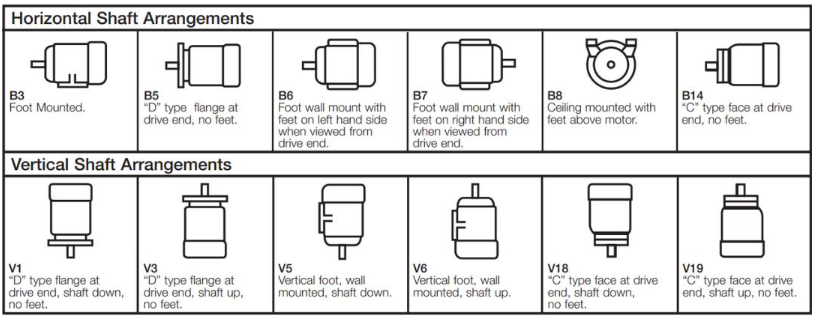
\includegraphics[width=0.8\textwidth]{assets/bouwvorm.png}
  \caption{Bouwvormen van motoren}
  \label{fig:bouwvorm.png}
 \end{figure}

\subsection{Motor Catalogus}
Het echt 'kiezen' van de motor doen we met een motorcatalogus, hierin zie je meerdere
gegevens die niet op de kenplaat staan, verschillende lastbedrijven, kipkoppels, geluid,
$\cdots$

\begin{figure}[H]
  \centering
  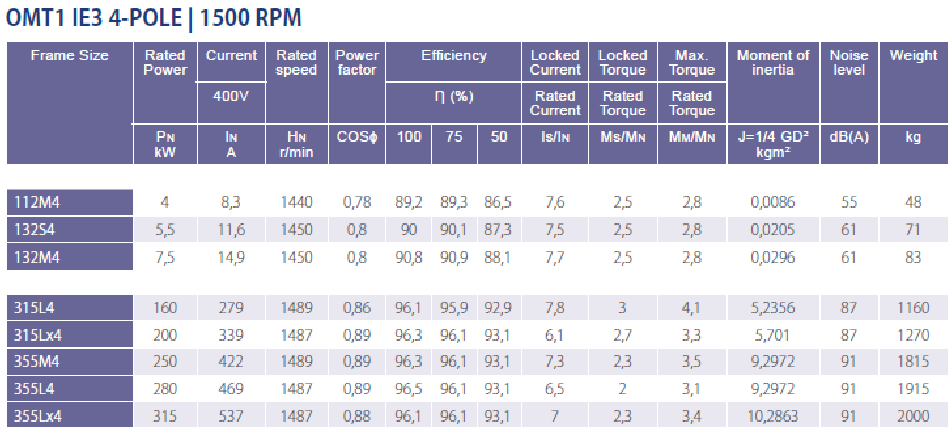
\includegraphics[width=0.8\textwidth]{assets/voorbeeldmotorcatalogus.png}
  \caption{Voorbeeld van een motorcatalogus}
  \label{fig:voorbeeldmotorcatalogus.png}
 \end{figure}

We zien hier ook die 'rated power', dit is meestal het belangrijkste gegeven dat je nodig
hebt om te kijken of de motor geschikt is voor je toepassing.
Daar bij het rendement zie je de efficientie voor vollast, deellast en halflast.
Zelfs de stroom bij blokkeren (stilstand) staat hier op.

\subsection{Motor dimensionering}
Dan gaan we nu kijken naar hoe we onze motor zelf kunnen dimensioneren, sommige dingen
bereken je zelf, sommige dingen hangen af van je toepassing.
Verschillende bepalende factoren zijn:

\begin{itemize}
    \item \textbf{Vermogen} van de motor, dit zelf hangt dan nog is af van de
    \textbf{snelheidsrange} en je \textbf{koppel} (\textit{nominaal, kip en 'houd' koppel
    }(dit is bij stilstand, vooral handig bij stappenmotoren gewoon))
    \item Directe aandrijving of via een \textbf{transmissie} (bvb.
    tandwielkast, riem, $\cdots$)
    \item \textbf{Werkingsregime} (S1, S2, $\cdots$)
    \item \textbf{Beschikbare voeding} (je kan bvb.
    een 1f of 3f voeding hebben van een bepaalde spanning)
    \item \textbf{Coupling} (mechanisch, hydraulisch, $\cdots$)
    \item \textbf{Mounting} (hangt dus eigelijk af van de \textbf{bouwvorm} van de motor)
    \item \textbf{Omgeving} (explosieveilig, stof, vocht, $\cdots$)
    \item \textbf{Prijs!}
\end{itemize}

\subsubsection{Voorbeeldoefening Roller}
Stel we hebben een toepassing waarbij we eigelijke een materiaal willen walsen met 2
rollers, we willen dan weten wat voor motor we nodig hebben.
Met de afmetingen en snelheden gegeven zoals in volgende figuur gaan we dan nu eens
bepalen wat voor motor we nodig hebben.

\begin{figure}[H]
  \centering
  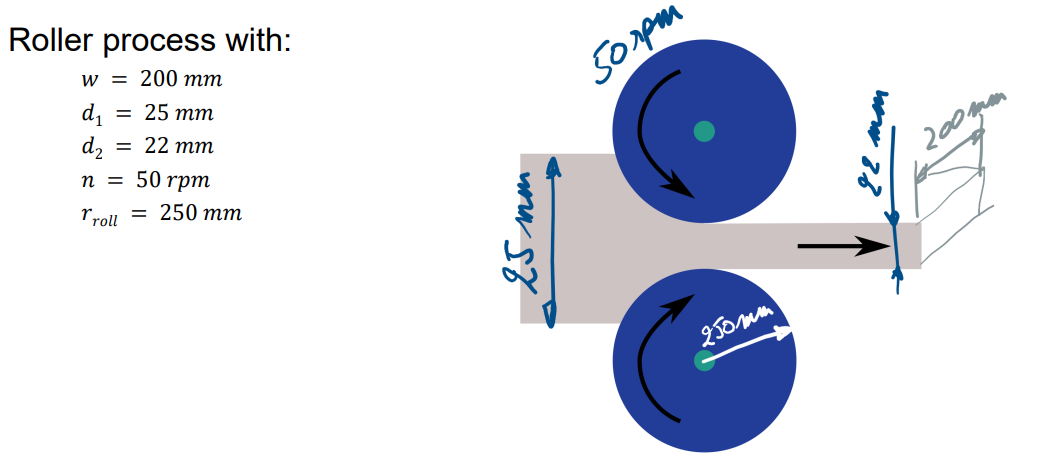
\includegraphics[width=0.8\textwidth]{assets/rolleroef.png}
  \caption{Roller oefening}
  \label{fig:rolleroef.png}
 \end{figure}

\begin{figure}[H]
  \centering
  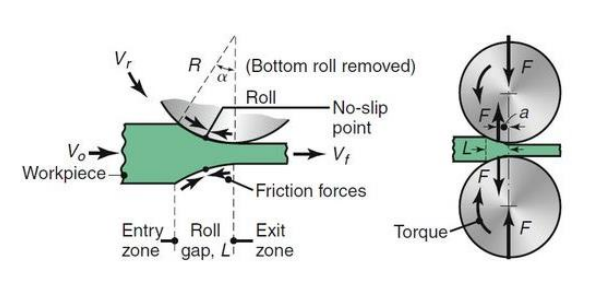
\includegraphics[width=0.6\textwidth]{assets/werkingroller.png}
  \caption{Krachtendiagram rollers}
  \label{fig:werkingroller.png}
 \end{figure}

De slides geven hier nog bij dat er een contact lengte is van 27.4mm (dit komt van
$L = \sqrt{R \cdot \Delta d} = \sqrt{250mm \cdot (25mm - 22mm)}$ maar moeten we niet
kennen) en een gemiddelde vloeispanning van 176 MPa.
Met een rare walskracht formule die we niet moeten kennen wordt een kracht van
$F = 962 kN$ gevonden en kan hiermee het koppel van de rollers bepaald worden:
\begin{align*}
    T_{roll} = F \cdot \frac{L}{2} = 962 kN \cdot \frac{27.4 mm}{2} = 13.2 kNm
\end{align*}
Dit is dus het koppel \textit{per} rol.
Als we beide rollers met dus dezelfde motor aandrijven dan is het totale vermogen nodig
voor die motor:
\begin{align*}
    P_{tot} = 2 \cdot T_{roll} \cdot \omega_{roll} = 2 \cdot 13.2 kNm \cdot 2\pi \cdot \frac{50 rpm}{60} = 138 kW
\end{align*}
Als we nu nog rekening houden met een rendement van 0.9 dan kunnen we dit theoretisch
mechanisch vermogen omzetten in elektrisch vermogen dat we nodig hebben:
\begin{align*}
    P_{el} = \frac{P_{tot}}{\eta} = \frac{138 kW}{0.9} = 153 kW
\end{align*}
We hebben dus een motor nodig van 153 kW, in de onderstaande catalogus komt dit overeen
met de rode omkaderde motor.
We zien hier wel dat deze een nominale snelheid van 993 tr/min heeft, dus hebben we een
overbrenging nodig.

\begin{figure}[H]
  \centering
  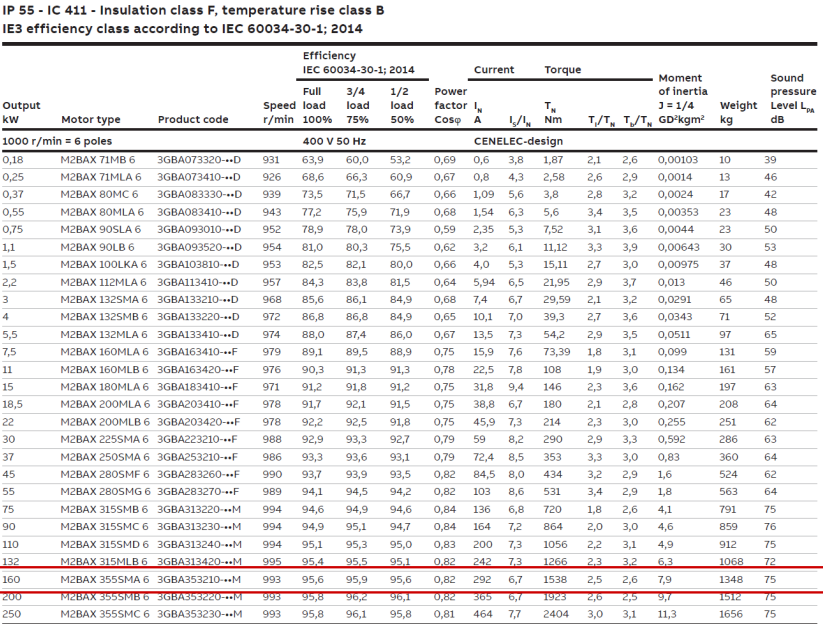
\includegraphics[width=0.6\textwidth]{assets/motorcatalogusroller.png}
  \caption{Motor Catalogus}
  \label{fig:motorcatalogusroller.png}
 \end{figure}

In een aandrijving zijn meerdere rendementen eigelijk, we hebben ons rendement van de
motor ($\eta_{mot}$), het rendement van de transmissie ($\eta_{tr}$) en het rendement van
de load ($\eta_{load}$).
Die van de motor zelf gebruiken we eigelijk niet om de motor te kiezen, we gebruiken die
van de load, dit is eigelijk het totale rendement.
Het echt weten van welk rendement je nodig hebt en wanneer behoort wel niet tot deze
cursus, dit is iets wat je ziet in het vak Dimensionering van Machines.
% Zorg dat dit in je preamble staat (waarschijnlijk al aanwezig):
% \usepackage{graphicx}
% \usepackage{tikz}
% \usetikzlibrary{shapes.geometric, arrows.meta, calc, positioning}

\begin{figure}[h]
\centering
\resizebox{\textwidth}{!}{%
\begin{tikzpicture}[
    font=\sffamily,
    circnode/.style={circle, draw=black, thick, minimum size=2.1cm,
        align=center, font=\sffamily\bfseries},
    blocknode/.style={rectangle, draw=black, thick, minimum width=1.0cm},
    loadnode/.style={rectangle, rounded corners=8pt, draw=black, thick,
        minimum width=2.7cm, minimum height=2cm,
        align=center, font=\sffamily\bfseries},
    Pbox/.style={rectangle, draw=black, fill=magenta!12,
        minimum width=1.2cm, minimum height=0.65cm, font=\small,
        align=center, inner sep=1pt},
    etabox/.style={rectangle, draw=black!70, fill=green!12,
        minimum width=1.2cm, minimum height=0.65cm, font=\small,
        align=center, inner sep=1pt},
]

% ---------- Bovenste rij: Grid - IM - Transmission (bovenste helft) ----------
\node[circnode, fill=orange!35]                (grid) at (0,3)   {Grid};
\node[circnode, fill=red!70!black, text=white] (im)   at (4.4,3) {IM};
\node[blocknode, fill=cyan!55!blue!35, minimum height=1.3cm] (trans1) at (7.6,3) {};

% ---------- Onderste rij: Transmission (onderste helft) - Mechanical load ----------
% trans2 zit vlak onder trans1, met een kleine gap (geen verbindingslijn ertussen)
\node[blocknode, fill=cyan!55!blue!35, minimum height=2cm] (trans2)
    at ($(trans1.south)+(0,-0.3cm-1cm)$) {};
\node[loadnode, fill=green!35] (load) at ($(trans2)+(4.2,0)$) {Mechanical\\load};

% Leader-lijn + label "Transmission" (wijst naar de gap tussen beide blokken)
\node[font=\small] (translabel) at ($(trans1.north)+(1.9,0.3)$) {Transmission};
\draw[-{Latex[length=2mm]}] (translabel.south west) -- ($(trans1.south)!0.5!(trans2.north)$);

% ---------- Verbindingen ----------
% Grid -- IM : elektrisch, driefasig (3 lijnen)
\foreach \dy in {-0.22,0,0.22}{
    \draw[thick] ($(grid.east)+(0,\dy)$) -- ($(im.west)+(0,\dy)$);
}
% IM -- Transmission (bovenste blok) : mechanische as (2 lijnen)
\foreach \dy in {-0.15,0.15}{
    \draw[thick] ($(im.east)+(0,\dy)$) -- ($(trans1.west)+(0,\dy)$);
}
% Transmission (onderste blok) -- Mechanical load : mechanische as (2 lijnen)
\foreach \dy in {-0.15,0.15}{
    \draw[thick] ($(trans2.east)+(0,\dy)$) -- ($(load.west)+(0,\dy)$);
}

% ---------- Vermogens (magenta) — netjes gecentreerd boven het midden van elke lijn ----------
\node[Pbox] at ($(grid.east)!0.5!(im.west)+(0,0.7)$)    {$P_{el}$};
\node[Pbox] at ($(im.east)!0.5!(trans1.west)+(0,0.7)$)  {$P_{mot}$};
\node[Pbox] at ($(trans2.east)!0.5!(load.west)+(0,0.7)$){$P_{tr}$};
\node[Pbox] at ($(load.north)+(0,0.7)$)                 {$P_{load}$};

% ---------- Rendementen (groen) — netjes gecentreerd onder elk blok ----------
\node[etabox] at ($(im.south)+(0,-0.7)$)    {$\eta_{mot}$};
\node[etabox] at ($(trans2.south)+(0,-0.7)$){$\eta_{tr}$};
\node[etabox] at ($(load.south)+(0,-0.7)$)  {$\eta_{load}$};

\end{tikzpicture}%
}
\caption{Efficiency motor $\leftrightarrow$ transmission $\leftrightarrow$ load}
\end{figure}

\subsubsection{Voorbeeldoefening Hoist {\color{red}(Dit kwam als meerkeuze op mijn
examen)}}
Nu kijken we naar een kraan die met een touw rol een last op tilt, er is hier een tandwiel
overbrenging aanwezig zoals we zien in volgende figuur:

\begin{figure}[H]
  \centering
  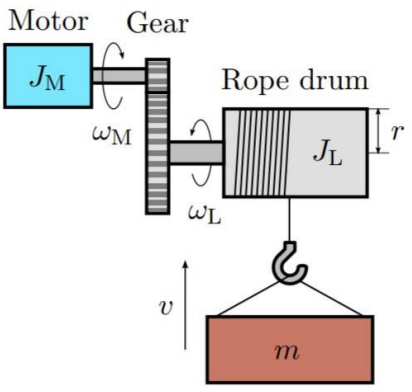
\includegraphics[width=0.4\textwidth]{assets/hoistoefening.png}
  \caption{Hoist Oefening}
  \label{fig:hoistoefening.png}
 \end{figure}

Volgende waardes zijn gegeven:

\begin{itemize}
    \item \textbf{m = 650 kg}
    $\rightarrow F_{load} = m \cdot g = 650 kg \cdot 9.81 m/s^2 = 6376.5 N$
    \item $\mathbf{h_{hoist} = 13 m}$
    \item $\mathbf{t_{hoist} = 30 s}$ 
    \newline
    Samen met de hoogte vinden we de arbeid geleverd door de last en dus het nodige
    vermogen met deze tijd:
    $W = F_{load} \cdot h_{hoist} = 6376.5 N \cdot 13 m = 82894.5 J$ en
    $P_{mass} = \frac{W}{t_{hoist}} = \frac{82894.5 J}{30 s} = 2763.15 W = 2.76 kW$ Ook
    vinden we de snelheid van de last:
    $v_{mass} = \frac{h_{hoist}}{t_{hoist}} = \frac{13 m}{30 s} = 0.433 m/s$
    \item $\mathbf{d_{drum} = 70 cm}$ 
    \newline
    Hiermee vinden we het koppel op de rol:
    $T_{drum} = F_{load} \cdot \frac{d_{drum}}{2} = 6376.5 N \cdot \frac{0.7 m}{2} = 2231.78 Nm$
    \item $\mathbf{l_{drum} = 4 m}$
    \item $\mathbf{\rho_{steel} = 7800\ kg/m^3}$
\end{itemize}

Met de snelheid van de massa kunnen we ook het toerensnelheid van die rol (drum) bepalen:
\begin{align*}
    n_{drum} = \frac{v_{mass}}{\pi \cdot d_{drum}} \cdot 60 = \frac{0.433 m/s}{\pi \cdot 0.7 m} \cdot 60 = 11.8 rpm (\omega_{drum} = \omega_{L} = 1.23 rad/s)
\end{align*}
Er wordt hier geen poolpaartal ofzo gegeven of berekend, ik denk dus dat het is dat je in
deze toepassing zowieso moet kiezen uit een 4 polige motor uit een catalogus die ik
zometeen ga tonen, deze motors hebben dus 4 polen en dus een nominale snelheid tussen de
1400rpm en 1500rpm, op voorand weet je dit niet altijd exact want je kiest nog geen motor.
We hebben hier dus wel al zowieso een overbrenging nodig want onze drum draait veel trager
dan de motor.
We gaan een gemiddelde nemen van 1450 rpm om de overbrengingsverhouding te bepalen:
\begin{align*}
  i = \frac{n_{mot}}{n_{drum}} = \frac{1450 rpm}{11.8 rpm} = 122.88
\end{align*}
Bij deze oefening gaan we van een rendement van 0.7 uit dus gaat een 3kW motor niet
voldoende zijn, we berekenen een vermogen voor de motor van:
\begin{align*}
    P_{mot} = \frac{P_{mass}}{\eta} = \frac{2.76 kW}{0.7} = 3.94 kW
\end{align*}
Dus kiezen we een 4kW motor uit de catalogus, deze heeft wel 1443 tr/min en een rendement
op vollast van 0.886 dus eigelijk moet je iteraties doen hiermee en dus opnieuw berekenen.

\begin{figure}[H]
  \centering
  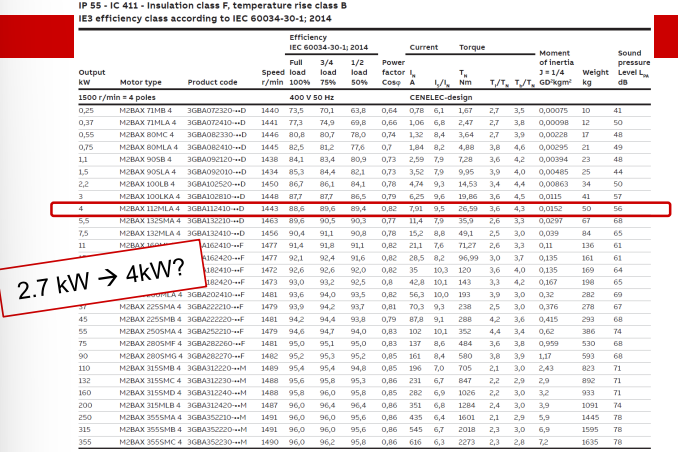
\includegraphics[width=0.6\textwidth]{assets/motorcatalogushoist.png}
  \caption{Motor Catalogus Hoist}
  \label{fig:motorcatalogushoist.png}
 \end{figure}

Maar 1 ding waar we nog geen rekening mee hebben gehouden is dat het hijstoestel niet
onmiddelijk op topsnelheid start en niet onmiddelijk stopt, het versnelt eerst, houdt een
tijdje de topsnelheid aan en vertraagt weer zoals we zien in volgende figuur:

\begin{figure}[H]
  \centering
  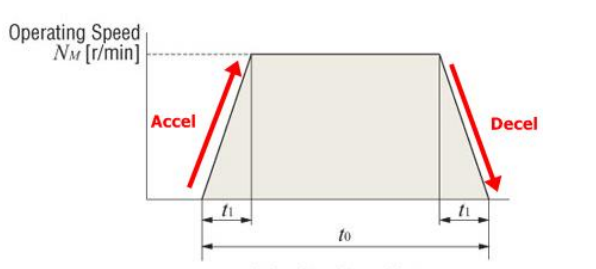
\includegraphics[width=0.6\textwidth]{assets/trapzeiumvormsnelheid.png}
  \caption{Trapzeiumvormige snelheid van de last bij een hijstoestel}
  \label{fig:trapzeiumvormsnelheid.png}
 \end{figure}

Die tijd om te versnellen en te vertragen is eigelijk niet meegegeven in onze opgave (deze
wordt bijna nooit meegegeven zelfs), in de praktijk nemen we dan zelf een realistische
waarde aan zoals $t_{acc} = t_{dec} = 2 s$.
Tijdens deze tijd legt de last wel minder afstand af dan bij die topsnelheid, dus om 13 m
in 30s te halen gaat onze snelheid iets hoger moeten liggen dan de eerder berekende
snelheid.
Als we zeggen dat onze beide driehoeken van die trapezium evenveel afstand afleggen als 1
rechthoekige blok in dus die 2s (niet 4!) aan de topsnelheid dan kunnen we de juiste
topsnelheid berekenen met:
\begin{align*}
 v_{top} = \frac{h_{hoist}}{t_{hoist} - t_{acc}} = \frac{13 m}{30 s - 2 s} = 0.464 m/s
\end{align*}
Met deze snelheid berekenen we het statisch (niet-versnellende) vermogen (rekening houden
met dat rendement terug):
\begin{align*}
 P_{stat} = \frac{F_{load} \cdot v_{top}}{\eta} = \frac{6376.5 N \cdot 0.464 m/s}{0.7} = 4.23 kW
\end{align*}
Dit is dus eigelijk een deel van ons totaal vermogen dat we nodig hebben, we hebben
namelijk ook nog een dynamisch vermogen nodig om de massa te versnellen.
Dit vermogen dient vooral om alle traagheidsmomenten van het systeem te versnellen, deze
hebben eigelijk een bepaald koppel nodig:
\begin{align*}
 T_{dyn} = J \cdot \alpha
\end{align*}
Al deze relevante traagheidsmomenten van de verschillende massas dus gaan wel
gereflecteerd/transformeerd moeten worden (geherleid) naar de motoras, dit wordt normaal
gedaan met de volgende formule:
\begin{align*}
 J_{x} = \frac{J_{load}}{i^2}
\end{align*}
Maar voor een lineair bewegende massa zoals hier is er een andere formule die we kunnen
gebruiken, namelijk:
\begin{align*}
    J_{x} = \frac{m \cdot v^2}{\omega^2}
\end{align*}
In ons geval hebben we drie bijdragen:

\begin{itemize}
 \item $\mathbf{J_{rotor}}$:
 Het traagheidsmoment van de motor zelf, deze kunnen we aflezen uit de motorcatalogus en
 bedraagt hier dus 0,0152 $kg m^2$
 \item $\mathbf{J_{drum}}$:
 Het traagheidsmoment van de rol, bij benadering is dit een volle stalen cillinder met de
 gegeven $\rho_{Steel}$, $r_{drum}$ en $l_{drum}$, dit traagheidsmoment wordt berekend
 met:
 \begin{align*}
 J_{drum} = \frac{1}{2} \cdot m_{drum} \cdot r_{drum}^2
 \end{align*}
  Met $m_{drum} = \rho_{steel} \cdot \pi \cdot r_{drum}^2 \cdot l_{drum}$.
  Die formule voor de cilinder komt uit deze tabel:
  \begin{figure}[H]
    \centering
    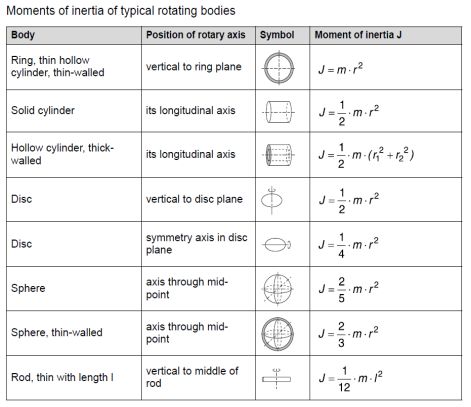
\includegraphics[width=0.4\textwidth]{assets/traagheidsmomenten.png}
    \caption{Tabel traagheidsmomenten van verschillende vormen}
    \label{fig:traagheidsmomenten.png}
   \end{figure}
 \item $\mathbf{J_{massa}}$:
 Het traagheidsmoment van de massa, dit is herleid naar de as van de drum (rol) en wordt
 berekend met:
    \begin{align*}
    J_{massa} = \frac{m_{massa} \cdot v_{top}^2}{\omega_{drum}^2} = m_{massa} \cdot r_{drum}^2 
    \end{align*}
    (Want $v_{top} = \omega_{drum} \cdot r_{drum}$)
\end{itemize}

Het optellen van deze traagheidsmomenten + het herleiden naar de motoras voor het
traagheidsmoment van de drum en de massa (rekening houdend met een rendement $\eta_{GB}$
van de tandwielkast) wordt dan als volgt gedaan:
\begin{align*}
    J_{tot} = J_{rotor} + \frac{J_{drum} + J_{massa}}{i^2 \cdot \eta_{GB}} = 0.105 kg m^2
\end{align*}
(Dat rendement is niet gegeven in deze oefening, gewoon de uitkomst van $J_{tot}$ staat op
de slides, op toledo staat er wel een gearbox efficiency van 90\% bij dezelfde oefening
als deze met iets andere gegevens)

De hoekversnelling van de motor $\alpha$ kunnen we berekenen met de volgende formule:
\begin{align*}
    \alpha = \omega_{top}/t_{acc} = 151.5 rad/s / 2 s = 75.8 rad/s^2
\end{align*}
Hiermee kunnen we dan het dynamisch koppel berekenen:
\begin{align*}
    T_{dyn} = J_{tot} \cdot \alpha = 0.105 kg m^2 \cdot 75.8 rad/s^2 = 7.96 Nm
\end{align*}
Het dynamisch vermogen dat we nodig hebben om de massa te versnellen is dan:
\begin{align*}
    P_{dyn} = T_{dyn} \cdot \omega_{top} = 7.96 Nm \cdot 151.5 rad/s = 1.21 kW
\end{align*}
Het werd wel niet verder uitgelegd op de slide maar dit resultaat is een eerste ruwere
doorrekening, na een iteratie is er gevonden voor dit vermogen dat het gelijk is aan 1.37
kW waardoor het optellen een totaal vermogen geeft van:
\begin{align*}
    P_{tot} = P_{stat} + P_{dyn} = 4.23 kW + 1.37 kW = 5.6 kW
\end{align*}
Dus een totaal koppel van:
\begin{align*}
    T_{tot} = \frac{P_{tot}}{\omega_{top}} = \frac{5.6 kW}{151.5 rad/s} = 36.6 Nm
\end{align*}
Uit de catalogus kiezen we nu echter voor een 5.5 kW motor, ons totaal koppel hierbij is
wel iets hoger dan ons nominaal koppel maar dat boeit niet want het kipkoppel is 2,6 keer
groter.

\begin{figure}[H]
  \centering
  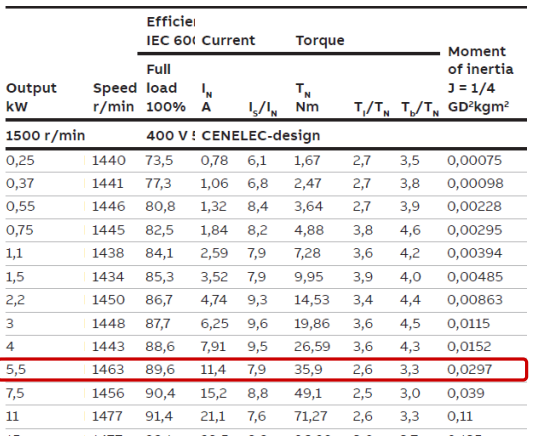
\includegraphics[width=0.5\textwidth]{assets/55kwmotorselectie.png}
  \caption{Motorcatalogus 5.5 kW motor}
  \label{fig:55kwmotorselectie.png}
 \end{figure}

\begin{warningbox}[5.5 kW motor terwijl we 5.6 kW nodig hebben?]
 Hoewel ons totaal vermogen berekend is op 5.6 kW, kiezen we toch een 5.5 kW motor uit de
 catalogus, dit is het nominaal vermogen, het is niet erg om hier even over te zitten
 (zoals dus tijdens die 2 seconden bij ons), we kunnen dit dus wel even overbelasten.
 Dit is een betere keuze dan een overgedimensioneerde motor te kiezen.
 Je moet dus ook controleren of die motor de korte piekbelasting van 36.6 Nm in ons geval
 aankan zonder continu op dat niveau te moeten draaien, wat het dus kan hier want de
 aanloop-/piekkoppel t.o.v.
 nominaal koppel verhouding is 2.6
\end{warningbox}

% ==================================================================

\newpage
